%! Author = JustinMa
%! Date = 5/27/25

\documentclass[12pt]{article}

% Packages
\usepackage{amsmath}
\usepackage{graphicx}
\usepackage{booktabs}
\usepackage[labelfont=it, textfont=it]{caption}
\usepackage{float}
\usepackage{tikz}
\usepackage{setspace}
\usepackage{times}
\usepackage{longtable}
\usepackage{siunitx}
\usepackage[margin=1in]{geometry}
\usepackage[colorlinks=true, linkcolor=blue, citecolor=blue, urlcolor=blue]{hyperref}

\doublespacing

% TikZ libraries and styles
\usetikzlibrary{shapes.geometric, arrows.meta, positioning, shadows}

\tikzset{
    layer/.style={
        rectangle,
        draw=black!80,
        rounded corners,
        minimum width=5cm,
        minimum height=0.6cm,
        text centered,
        text width=7cm,
        font=\small,
        drop shadow,
        fill=#1
    },
    arrow/.style={
        -{Stealth[length=2mm]},
        thick,
        shorten >=2pt,
        shorten <=2pt
    }
}

\title{Investigating Overfitting in Convolutional Neural Networks}\date{}

\begin{document}

    \maketitle

    \section*{1 Introduction}

    Neural networks are a form of machine learning models, inspired by how the human brain
    processes information. They have become increasingly prevalent in our developing world, providing
    powerful and unique solutions to a wide variety of problems. However, with power also comes risk,
    as training a neural network too much on a small dataset can cause overfitting. Overfitting occurs
    when a model learns the training data too well by essentially memorizing it, causing it to perform
    well on data in its training set but poorly on test data (data that were not in the training set).
    While it might seem that simply increasing a model’s size would always boost accuracy by allowing it to
    capture more patterns, extra parameters often give the network enough capacity to store the training set
    outright when the training set is small, allowing it to overfit. Smaller networks, by contrast, are forced to find the underlying patterns
    in the data because of their limited size. In this study, we investigate whether increasing the number of
    parameters in a convolutional neural network leads to greater overfitting when trained on a small dataset, as
    measured by the difference between its accuracy on the training dataset and the test dataset.

    \section*{2 Statistical Question}

    Does increasing the number of parameters in a fixed CNN architecture cause a greater difference
    between training and testing accuracy?

    \noindent\textbf{Hypotheses:}\newline
    \centerline{$H_0: \beta = 0$} \newline
    \centerline{$H_a: \beta > 0$} \newline
    Where $\beta$ is the true slope of the population least‐squares regression line that relates number
    of parameters of the model to the difference in accuracy of the model on the train dataset and the
    test dataset (train - test).

    \section*{3 Data Collection}

    We trained 150 convolutional models, each on the same randomly selected small subset of 100 images
    from the Canadian Institute For Advanced Research - 10 dataset (CIFAR-10), which consists of 32x32 color images each labeled with one of ten classes (e.g., plane, boat, etc).
    % Each model had the same architecture, with the only difference between them being the number of parameters (\textit{see Figure 1 below}).
    The training dataset was constructed through stratified random sampling by randomly selecting 10 of each class of image, ensuring that it is representative of the entire dataset.
    The number of filters and neurons were varied between models in a way such that the sizes of the models (in parameter count) were roughly uniformly distributed, ranging from approximately 1m to 25m parameters.
    The architecture and the ratio of layer sizes were kept consistent between each model, ensuring that the only difference between them was the number of parameters (\textit{see Figure 1 below}).
    On the initialization of each model, the values of the parameters for that model were randomly set, so each model can be seen as randomly
    selected from all possible models of their respective size and architecture before training, ensuring the experiment is statistically valid.
    All of the above precautions aimed to eliminate confounding with other variables, ensuring that any change in the accuracy of the models was actually caused by the change in parameter count.
    We controlled the parameter count by multiplying the amount of filters for the Conv2D layers and the amount of neurons
    for the hidden Dense layers by a scalar factor, $n$.

    \begin{figure}[H]
        \begin{center}
            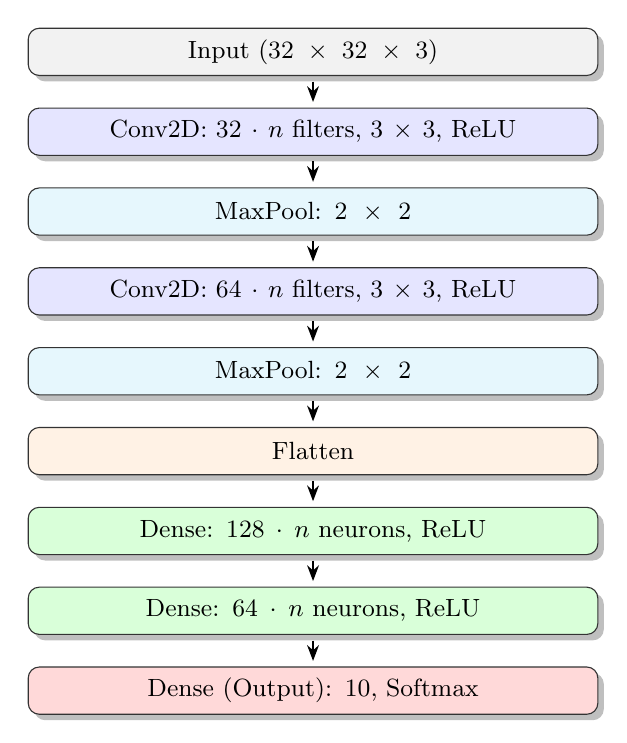
\begin{tikzpicture}[node distance=4mm and 0mm]
                \node[layer=gray!10]                     (input)  {Input $(32\times32\times3)$};
                \node[layer=blue!10,  below=of input]    (conv1)  {Conv2D: $32\cdot n$ filters, $3\times3$, ReLU};
                \node[layer=cyan!10,  below=of conv1]    (pool1)  {MaxPool: $2\times2$};
                \node[layer=blue!10,  below=of pool1]    (conv2)  {Conv2D: $64\cdot n$ filters, $3\times3$, ReLU};
                \node[layer=cyan!10,  below=of conv2]    (pool2)  {MaxPool: $2\times2$};
                \node[layer=orange!10,below=of pool2]    (flat)   {Flatten};
                \node[layer=green!15, below=of flat]    (dense1) {Dense: $128\cdot n$ neurons, ReLU};
                \node[layer=green!15, below=of dense1]  (dense2) {Dense: $64\cdot n$ neurons, ReLU};
                \node[layer=red!15,   below=of dense2]  (output) {Dense (Output): 10, Softmax};

                \draw[arrow] (input)  -- (conv1);
                \draw[arrow] (conv1)  -- (pool1);
                \draw[arrow] (pool1)  -- (conv2);
                \draw[arrow] (conv2)  -- (pool2);
                \draw[arrow] (pool2)  -- (flat);
                \draw[arrow] (flat)   -- (dense1);
                \draw[arrow] (dense1) -- (dense2);
                \draw[arrow] (dense2) -- (output);
            \end{tikzpicture}
            \caption{General Architecture of Our Models}
        \end{center}
        \label{fig:architecture}
    \end{figure}

    \noindent Each model was trained for 100 epochs on the randomly selected subset of 100 images, then evaluated
    on the full test set of the CIFAR-10 dataset, made up of 10,000 images. The difference between the train and test accuracy (train - test) was then
    computed for each model and graphed on a scatter plot with the $x$-axis
    as parameter count and the $y$-axis as the difference between train and test accuracy for each model.

    \section*{4 Data Display}
    \begin{figure}[H]
        \centering
        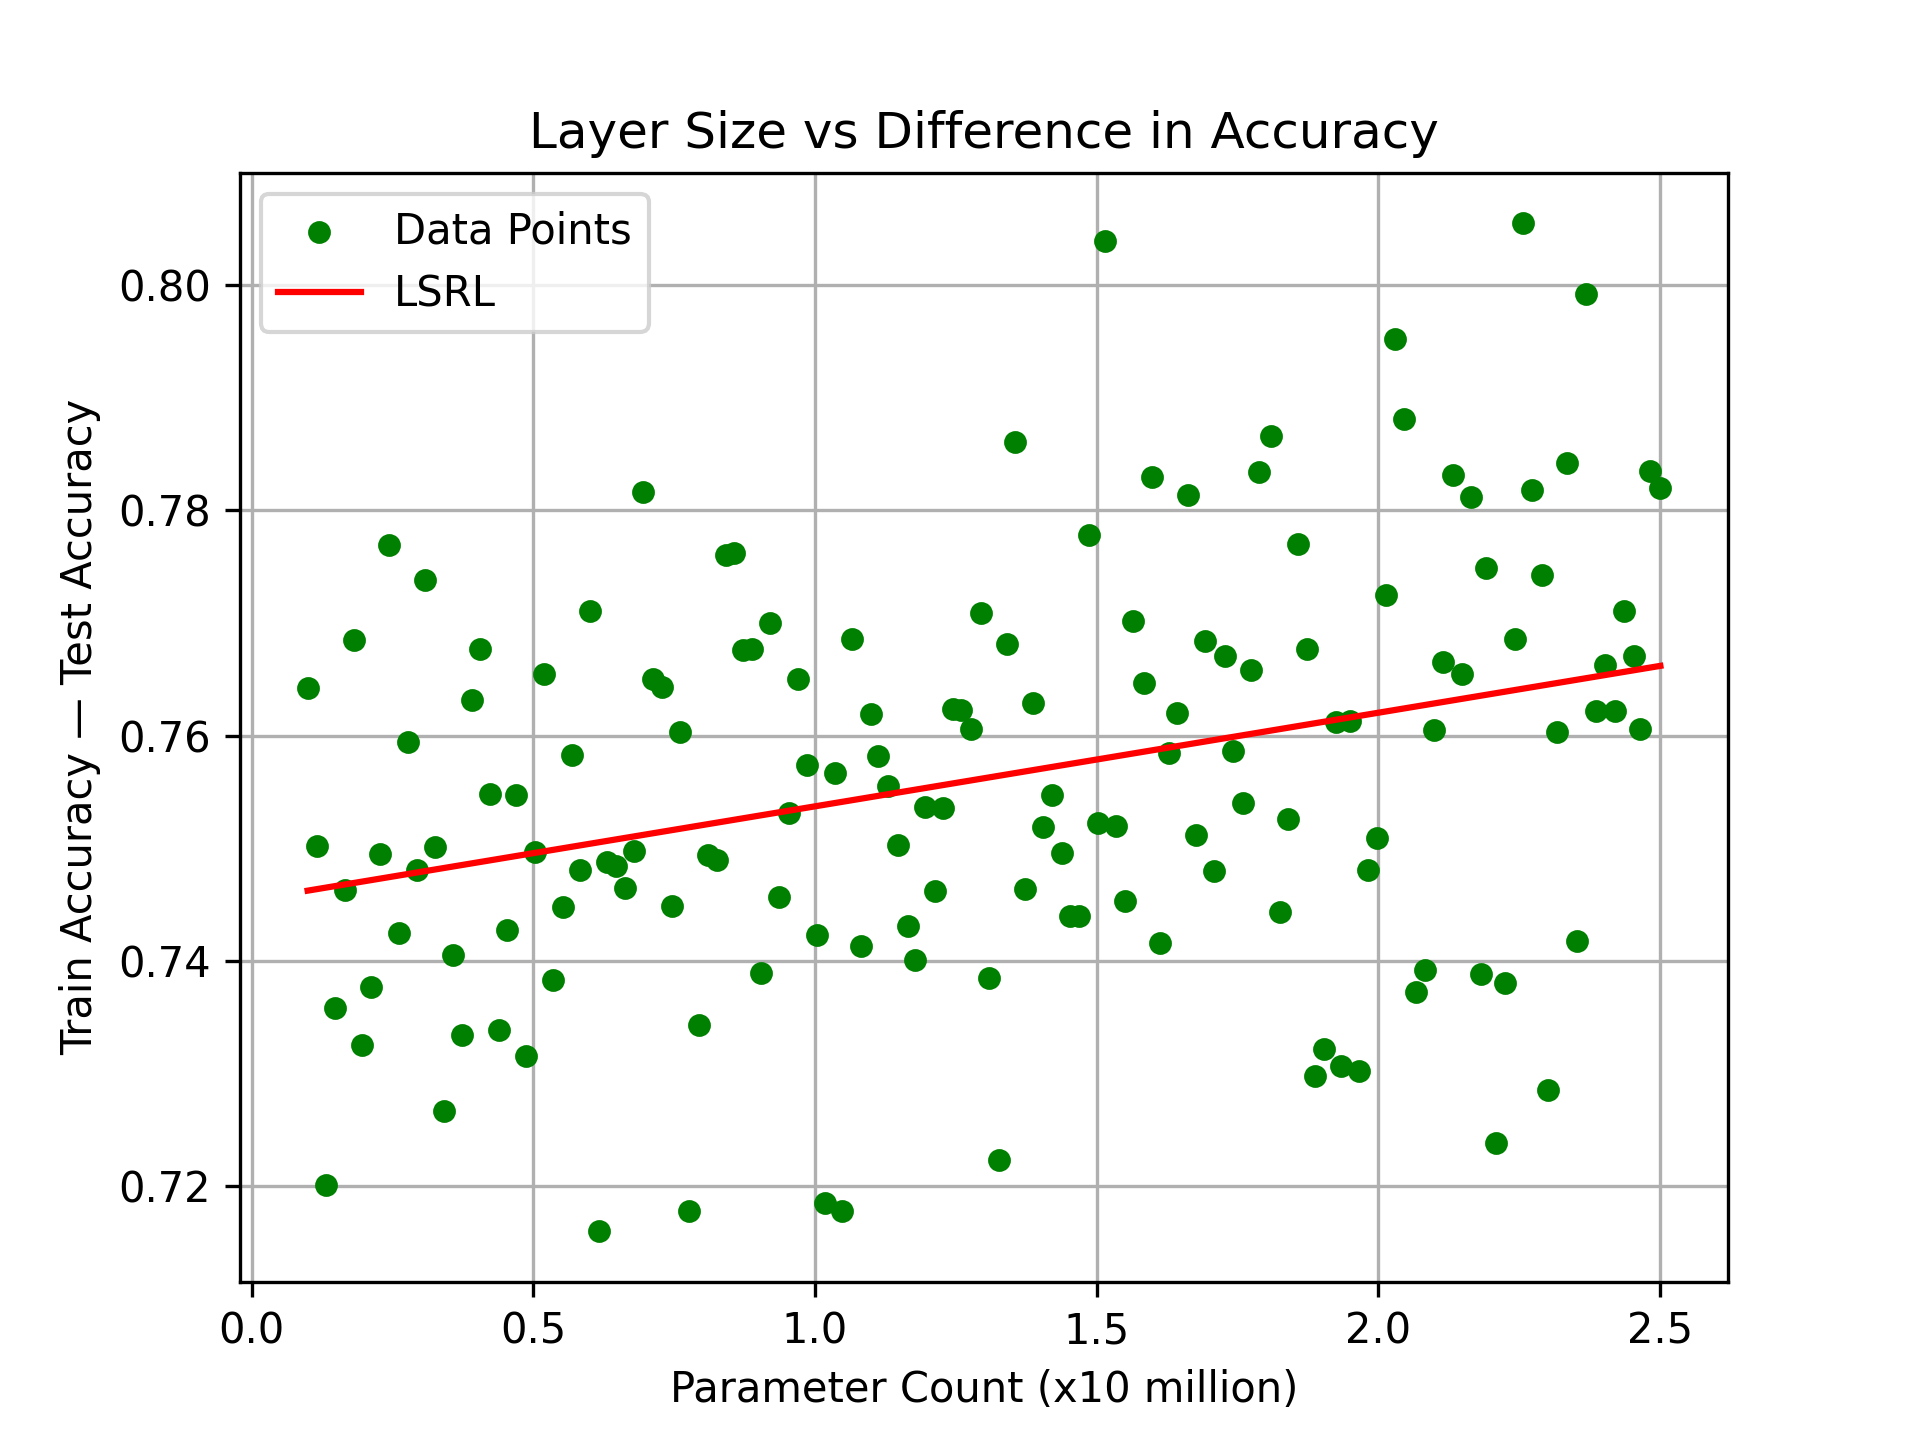
\includegraphics[width=1\textwidth]{Images/Scatter}
        \caption{Scatterplot of Parameter Count vs. Difference in Train and Test Accuracy (Train - Test)}
        \label{fig:scatterplot}
    \end{figure}

    \begin{table}[ht]
        \centering
        \begin{tabular}{|l|r|r|}
            \hline
            Predictor & Coef & SE Coef \\
            \hline
            Constant & 0.7454 &  \\
            Param Count (x10 mil)   & 0.0083 & 0.0020 \\
            \hline
            \multicolumn{2}{|l|}{$S = 0.01703$} & R-Sq = 10.37\% \\
            \hline
        \end{tabular}
        \caption{Regression Summary}
        \label{tab:minitab}
    \end{table}

    \noindent
    Based on the scatter plot (\textit{\autoref{fig:scatterplot}}) and the correlation coefficient of $r=\sqrt{0.1037}=0.3220$ (\textit{from \autoref{tab:minitab}}), there appears to be a weak,
    positive, linear relationship between parameter count and difference between train and test accuracy (train - test).
    There appear to be a few possible high outliers above $x =$ 1.5 million parameters
    and a few possible low outliers above $x = 0.5$ million parameters.
    \begin{figure}[H]
        \centering
        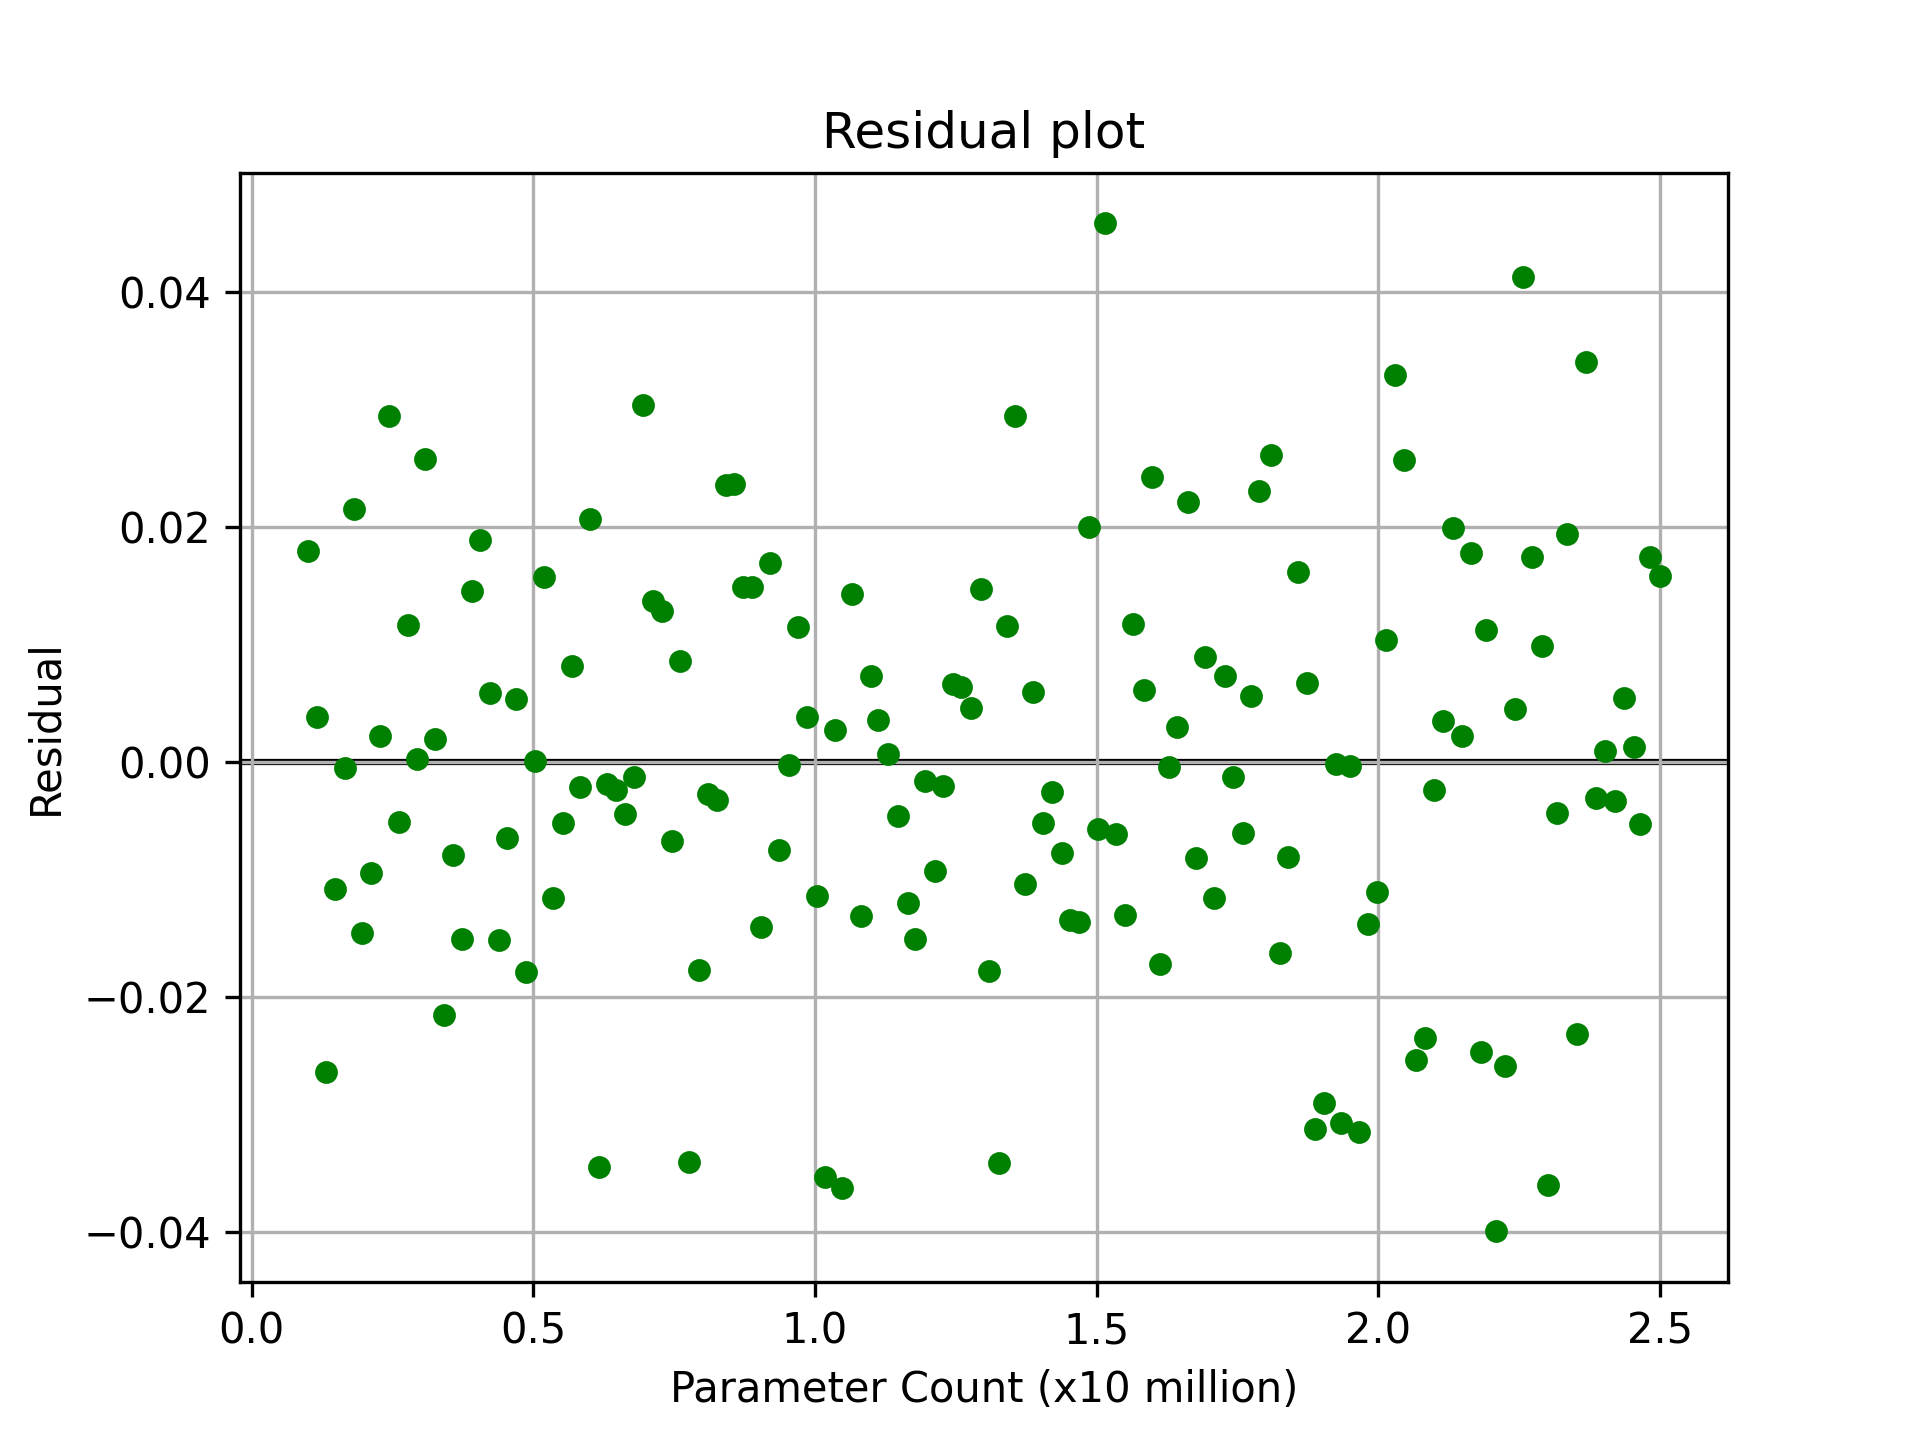
\includegraphics[width=0.6\textwidth]{Images/Resid}
        \caption{Residual Plot (Parameter Count vs. Residuals)}
        \label{fig:residuals}
    \end{figure}
    \noindent Because the residual plot (\textit{\autoref{fig:residuals}}) appears to have no form and because the standard
    deviation of the residuals $S$ (\textit{from \autoref{tab:minitab}}) is small ($0.01703$), the graphical display seems to
    indicate that the null hypothesis will be rejected.
    \begin{figure}[H]
        \centering
        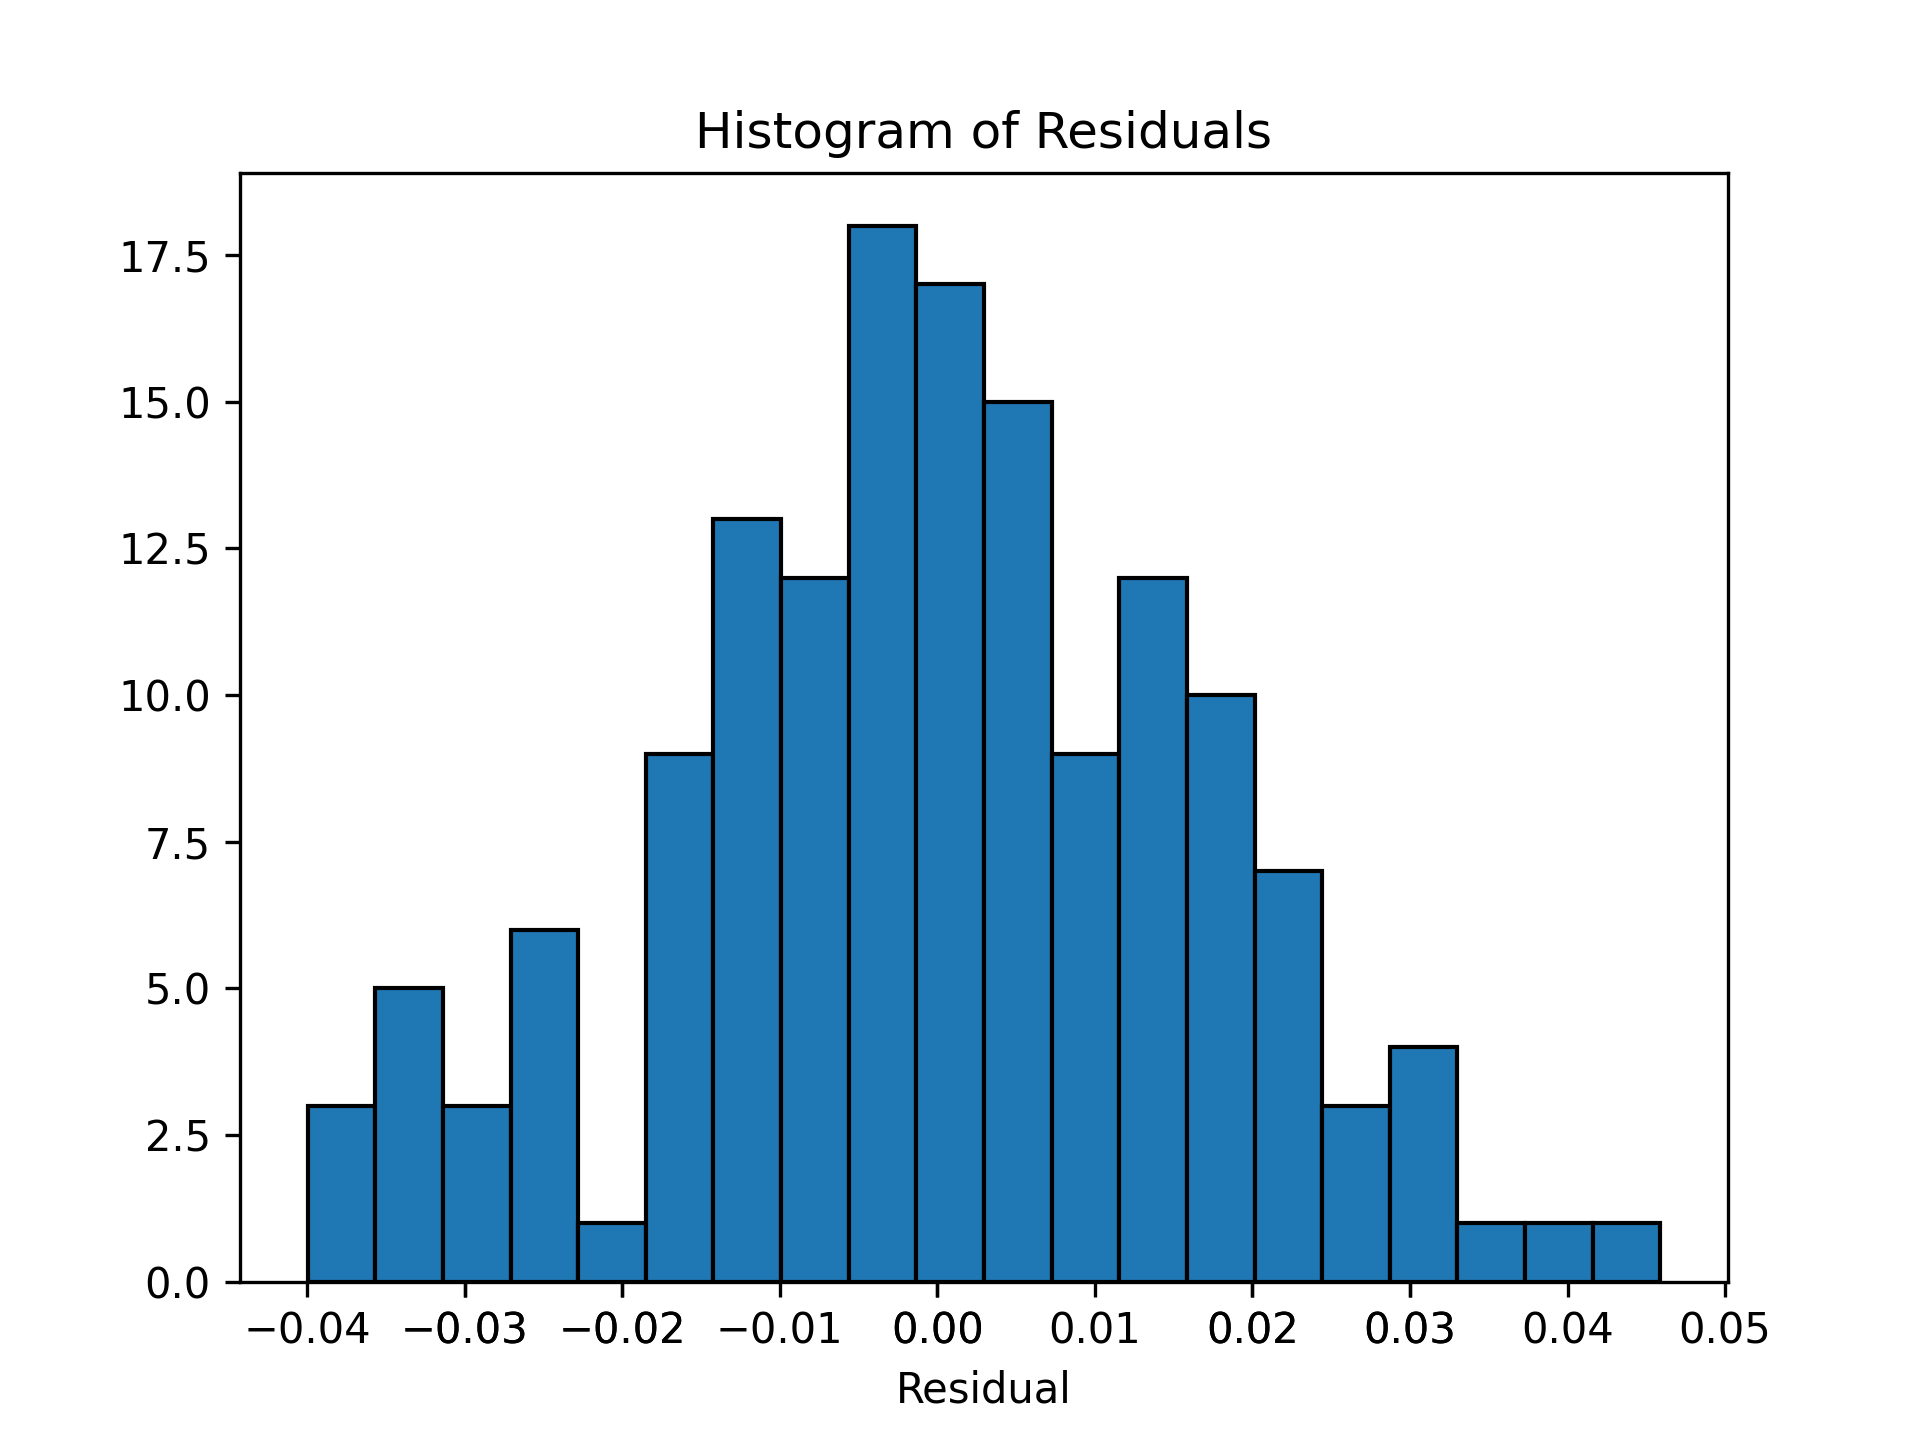
\includegraphics[width=0.6\textwidth]{Images/Resid Hist}
        \caption{Histogram of Residuals}
        \label{fig:residual_hist}
    \end{figure}
    \noindent The histogram of the residuals appears to be approximately symmetric, with a median around 0 and a range of
    $0.05-(-0.04)=0.09$. There does not appear to be any strong skew or outliers.

    \section*{5 Data Analysis}

    We conducted a $t$-test for the population slope $\beta$ of the least-squares regression line that relates the number of parameters in a model trained on a randomly selected 100-image subset of the CIFAR-10 dataset to the difference between its accuracy on training and test data (Train Accuracy $-$ Test Accuracy).

    \subsection*{5.1 Condition Check}

    \begin{quote}

    \textbf{5.1.1 Linear}

    The scatterplot of the data (\textit{\autoref{fig:scatterplot}}) shows a clear linear trend, and the residual plot (\textit{\autoref{fig:residuals}}) shows no remaining curved pattern.
    Therefore, the linearity condition is satisfied.

    \textbf{5.1.2 Independent}

    Each model was trained independently with no interaction between runs. Thus, the independence condition is met by the design of the experiment.

    \textbf{5.1.3 Normal}

    The histogram of the residuals (\textit{\autoref{fig:residual_hist}}) shows no strong skew and no obvious outliers,
    so the normality condition is met.

    \textbf{5.1.4 Equal Variance}

    The residual plot (\textit{\autoref{fig:residuals}}) shows shows no noticeable $<$ or $>$ shape, so the equal variance condition is satisfied.

    \textbf{5.1.5 Random}

    The parameters of the model were randomized on initialization, so each model can be seen as randomly selected from the population
    of models of the same size and structure.

    \end{quote}

    \subsection*{5.2 Calculations}

    \subsubsection*{5.2.1 Standard Error}

    We used the following equation to calculate the Standard Error $SE_\beta$ of the slope $\beta$:
    \[
        \mathrm{SE}_{\beta}
        =
        \frac{
            \displaystyle S
        }{
            \displaystyle S_x \sqrt{n - 1}
        }
    \]
    \noindent We need the standard deviation of the residuals and of the parameter counts to find $SE_\beta$, which we found like this:
    \begin{align*}
        \mathrm{S} &=
        \sqrt{
            \frac{
                \sum_{i=1}^n (y_i - \hat{y}_i)^2
            }{
                n - 2
            }
        } \\[1em]
        \mathrm{S}_x &=
        \sqrt{
            \frac{
                \sum_{i=1}^n (x_i - \bar{x})^2
            }{
                n - 1
            }
        }
    \end{align*}
    \noindent After plugging in all of the data from the 150 models, we got $S = 0.01703$ and $S_x = 0.6972$.
    Now we can use those to find $SE_\beta$:
    \[
        \mathrm{SE}_{\beta}
        =
        \frac{
            \displaystyle 0.01703
        }{
            \displaystyle 0.6972 \sqrt{150 - 1}
        }
        =
        0.002008
    \]

    \subsubsection*{5.2.2 $t$-statistic}
    \noindent And now we can find the $t$-statistic, which represents how many standard deviations away our sample slope $b$ is from the population slope $\beta$ on the sampling distribution, assuming that $\beta=0$:
    \begin{gather*}
        \mathrm{t} = \frac{b}{SE_\beta} \\[1em]
        \mathrm{t} = \frac{0.008312}{0.002008} = 4.139
    \end{gather*}

    \subsubsection*{5.2.3 $p$-value}
    \noindent Now that we have the $t$-statistic, we can use it to find the $p$-value, which represents the probability of getting a test statistic
    of $4.139$ or higher, assuming that the population slope $\beta$ is $0$. Because we have 150 data points, we have $150 - 2 = 148$ degrees of freedom.
    Thus, we calculate the $p$-value by finding the amount of area under a $t$-distribution with 148 degrees of freedom, above $t=4.139$. The graph below demonstrates this:

    \begin{figure}[H]
        \centering
        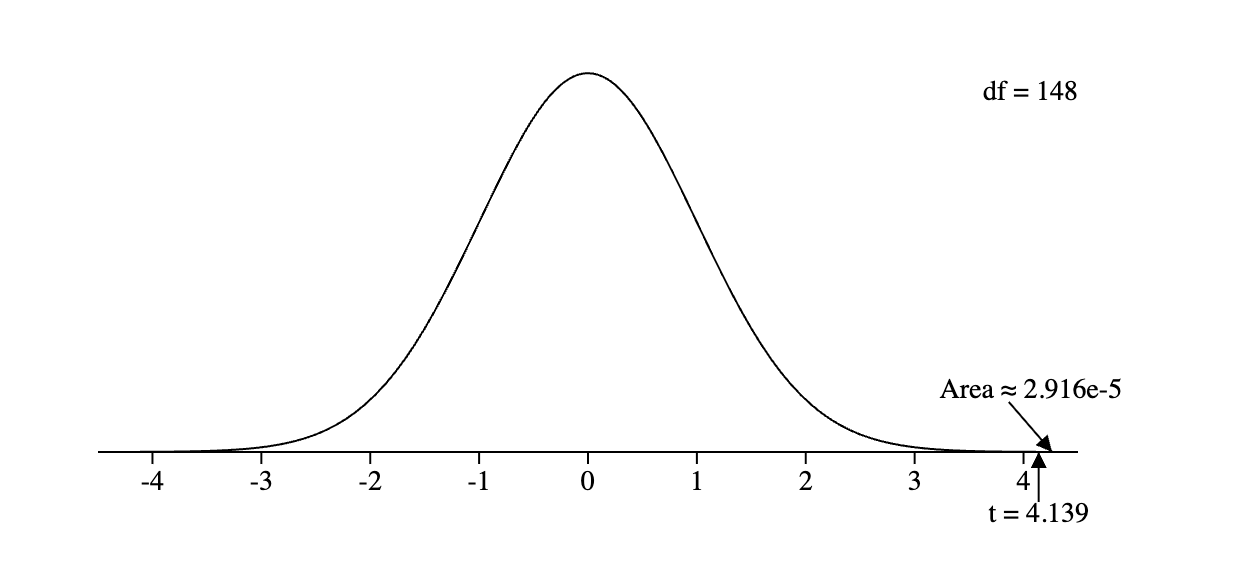
\includegraphics[width=0.7\textwidth]{Images/tdistribution}
        \caption{p-value calculation on a t-distribution with df = 148}
        \label{fig:t_dist}
    \end{figure}

    \noindent Based on the area under the curve in \textit{\autoref{fig:t_dist}} above $t=4.139$, our $p$-value is $2.916\cdot10^{-5}$.

    \section*{6 Conclusion}

    The $p$-value of $2.916\cdot10^{-5}$ indicates that, assuming that the population slope $\beta=0$, there is around a
    $0.002916\%$ probability of getting a sample slope as great or greater than our sample slope of $0.008312$, in a sample of
    150 randomly selected models from the population of convolutional models of our structure and of size 1 million parameters to 25 million parameters, trained
    on a randomly selected subset of 100 images from the CIFAR-10 train dataset and tested on the full test dataset of CIFAR-10.
    Because the $p$-value of $2.916\cdot10^{-5}$ is less than $\alpha=0.05$, we reject the null hypothesis, which states that the population slope $\beta$
    of the least-squares regression line that relates parameter count to difference in train and test accuracy (train - test) is $0$,
    in the population defined above.
    The data do provide convincing evidence that the population slope $\beta$ is greater than $0$, and that there is a positive correlation between
    parameter count and difference between train and test accuracy (train - test) in the population defined above. Thus, for that population, we can conclude that
    increasing the number of parameters in the model does indeed cause overfitting.


    \section*{7 Reflection}

    In our project, we aimed to determine whether increasing the parameter count of convolutional models of a specific structure caused the model to overfit,
    or essentially memorize the train dataset and perform well on images from that set but poorly on newly introduced images. We ensured equal representation
    of images of different classifications by randomly sampling by strata, with each strata being a group of images with the same classification.
    By keeping the structure of the models and the dataset on which they were trained on constant, as well as randomizing the parameters of the models
    on initialization, we prevented confounding with other variables, allowing us to establish a cause-and-effect relationship between parameter count
    and difference between train and test accuracy (train - test). Through a $t$-test for the population slope, we found that there is a positive relationship
    between parameter count and difference between train and test accuracy (train - test), and thus that increasing parameter count increases the difference and causes overfitting.

    \bigskip\noindent We could have potentially made a Type I error, because we rejected the null hypothesis. If we had made a Type I error,
    that would mean that we found convincing evidence that increasing the parameter count of the model between 1m and 25m parameters
    caused overfitting, when in reality it didn't. A potential consequence of this would be that we would only use models with less than 1 million parameters,
    believing that models larger than 1 million parameters would perform worse on the test dataset, losing the potential
    of getting better accuracy by using larger models.

    \bigskip\noindent However, our design included many limitations that could be addressed in future experiments.
    We only trained models with 1m to 25m parameters, which means we can only generalize to models of these sizes.
    In the future, we could conduct tests with a wider range of parameter sizes, which would allow us to generalize our results to a wider range of model sizes or potentially reveal a new trend with larger parameter sizes.

    \bigskip\noindent Another major limitation was the compute time required. Despite training relatively simple models on a small dataset, it took over two hours to train all 150 models.
    If we wanted to scale the experiment up with more complex models or larger datasets, the compute time required could make the experiment impractical.
    In the future, we could optimize the experiment by training the models for less epochs or using less models, although this would decrease the power of the test.

    \bigskip\noindent Finally, our results are only applicable to models of the specific architecture we used on a 100 image subset of the CIFAR-10 dataset, which is not useful to many people training neural networks.
    If we wanted the test to be more useful in helping people decide the size of their models, we could perform an experiment on different model architectures and datasets, allowing a broader generalization.



%    In the future, we could conduct tests beyond our current models architecture and our current parameter range,
%    to generalize to a larger population or find different trends. It is possible that as model size increases past
%    25 million parameters, that the difference in test and train accuracy could stop increasing and instead start decreasing.
%    We could also conduct tests with larger training datasets and see if the slope lowers as the training dataset size increases (because overfitting generally happens on small training datasets).
%    In the future we could also generalize our test to
    \clearpage
    \appendix
    \textbf{Appendix: Raw Data}
    \addcontentsline{toc}{section}{Appendix: Raw Data}

    \begingroup
    \scriptsize
    \setlength{\tabcolsep}{2pt}       % tighten column separation

    \begin{longtable}{@{}
        S[table-format=8.0] c
        S[table-format=8.0] c
        S[table-format=8.0] c
        S[table-format=8.0] c
        S[table-format=8.0] c
        S[table-format=8.0] c @{}}
        \caption{Raw Data: Parameter Count vs.\ Train–Test Accuracy Difference}\\
        \toprule
        \textbf{Param.} & \textbf{Acc.} & \textbf{Param.} & \textbf{Acc.} &
        \textbf{Param.} & \textbf{Acc.} & \textbf{Param.} & \textbf{Acc.} &
        \textbf{Param.} & \textbf{Acc.} & \textbf{Param.} & \textbf{Acc.}\\
        \midrule
        \endfirsthead

        \toprule
        \multicolumn{12}{c}{\textbf{(continued)}}\\\midrule
        \multicolumn{2}{c}{\textbf{Col 1}} & \multicolumn{2}{c}{\textbf{Col 2}} &
        \multicolumn{2}{c}{\textbf{Col 3}} & \multicolumn{2}{c}{\textbf{Col 4}} &
        \multicolumn{2}{c}{\textbf{Col 5}} & \multicolumn{2}{c}{\textbf{Col 6}} \\
        \textbf{Param.} & \textbf{Acc.} & \textbf{Param.} & \textbf{Acc.} &
        \textbf{Param.} & \textbf{Acc.} & \textbf{Param.} & \textbf{Acc.} &
        \textbf{Param.} & \textbf{Acc.} & \textbf{Param.} & \textbf{Acc.}\\
        \midrule
        \endhead

        \bottomrule
        \endfoot

        \num{991995}&0.7642  & \num{1156636}&0.7502  & \num{1314120}&0.7201  &
        \num{1481652}&0.7358  & \num{1653866}&0.7463  & \num{1817930}&0.7685  \\
        \num{1964108}&0.7325  & \num{2122007}&0.7377  & \num{2279711}&0.7495  &
        \num{2443067}&0.7769  & \num{2612075}&0.7425  & \num{2779778}&0.7594  \\
        \num{2928578}&0.7481  & \num{3083068}&0.7738  & \num{3247185}&0.7501  &
        \num{3409755}&0.7267  & \num{3574350}&0.7405  & \num{3736748}&0.7334  \\
        \num{3908963}&0.7632  & \num{4058757}&0.7677  & \num{4231690}&0.7548  &
        \num{4387487}&0.7339  & \num{4537211}&0.7427  & \num{4689447}&0.7547  \\
        \num{4872926}&0.7316  & \num{5030648}&0.7497  & \num{5190882}&0.7655  &
        \num{5353628}&0.7383  & \num{5518886}&0.7448  & \num{5686656}&0.7583  \\
        \num{5825435}&0.7481  & \num{5997767}&0.7711  & \num{6162250}&0.7160  &
        \num{6304105}&0.7488  & \num{6472707}&0.7484  & \num{6620711}&0.7465  \\
        \num{6793468}&0.7498  & \num{6942372}&0.7816  & \num{7119248}&0.7650  &
        \num{7274427}&0.7643  & \num{7455458}&0.7449  & \num{7611411}&0.7603  \\
        \num{7760207}&0.7178  & \num{7947148}&0.7343  & \num{8108136}&0.7494  &
        \num{8261687}&0.7490  & \num{8413707}&0.7760  & \num{8570111}&0.7762  \\
        \num{8724930}&0.7676  & \num{8884187}&0.7677  & \num{9041805}&0.7389  &
        \num{9203915}&0.7700  & \num{9364332}&0.7457  & \num{9529295}&0.7531  \\
        \num{9692511}&0.7650  & \num{9860327}&0.7574  & \num{10026342}&0.7423 &
        \num{10183690}&0.7185 & \num{10352393}&0.7567 & \num{10480242}&0.7178 \\
        \num{10654715}&0.7686 & \num{10813533}&0.7413 & \num{10990748}&0.7619 &
        \num{11122467}&0.7582 & \num{11298745}&0.7555 & \num{11465740}&0.7503 \\
        \num{11644706}&0.7431 & \num{11780277}&0.7401 & \num{11950780}&0.7537 &
        \num{12133478}&0.7462 & \num{12271857}&0.7536 & \num{12445868}&0.7624 \\
        \num{12586011}&0.7623 & \num{12773485}&0.7606 & \num{12951004}&0.7709 &
        \num{13093955}&0.7385 & \num{13269953}&0.7223 & \num{13399368}&0.7681 \\
        \num{13544767}&0.7861 & \num{13727548}&0.7464 & \num{13874711}&0.7629 &
        \num{14055863}&0.7519 & \num{14204772}&0.7547 & \num{14391938}&0.7496 \\
        \num{14526700}&0.7440 & \num{14678075}&0.7440 & \num{14864381}&0.7778 &
        \num{15017502}&0.7522 & \num{15155155}&0.8039 & \num{15348460}&0.7520 \\
        \num{15504047}&0.7453 & \num{15643907}&0.7702 & \num{15836226}&0.7647 &
        \num{15977573}&0.7830 & \num{16119548}&0.7416 & \num{16278987}&0.7585 \\
        \num{16422292}&0.7620 & \num{16623490}&0.7814 & \num{16768300}&0.7512 &
        \num{16930907}&0.7684 & \num{17077047}&0.7480 & \num{17277956}&0.7671 \\
        \num{17425583}&0.7586 & \num{17591340}&0.7540 & \num{17740297}&0.7658 &
        \num{17889882}&0.7834 & \num{18099850}&0.7866 & \num{18250940}&0.7443 \\
        \num{18402658}&0.7526 & \num{18572987}&0.7770 & \num{18726035}&0.7677 &
        \num{18879711}&0.7298 & \num{19034015}&0.7322 & \num{19246091}&0.7612 \\
        \num{19344507}&0.7307 & \num{19500695}&0.7613 & \num{19657511}&0.7302 &
        \num{19814955}&0.7481 & \num{19973027}&0.7509 & \num{20131727}&0.7725 \\
        \num{20291055}&0.7952 & \num{20451011}&0.7881 & \num{20670818}&0.7372 &
        \num{20832261}&0.7392 & \num{20994332}&0.7605 & \num{21157031}&0.7665 \\
        \num{21320358}&0.7831 & \num{21484313}&0.7655 & \num{21648896}&0.7812 &
        \num{21814107}&0.7388 & \num{21918875}&0.7749 & \num{22085111}&0.7238 \\
        \num{22251975}&0.7380 & \num{22419467}&0.7686 & \num{22567754}&0.8055 &
        \num{22736428}&0.7818 & \num{22905730}&0.7743 & \num{23008186}&0.7285 \\
        \num{23178495}&0.7603 & \num{23349432}&0.7842 & \num{23520997}&0.7418 &
        \num{23693190}&0.7992 & \num{23866011}&0.7622 & \num{24018998}&0.7663 \\
        \num{24193001}&0.7622 & \num{24367632}&0.7711 & \num{24542891}&0.7671 &
        \num{24654011}&0.7606 & \num{24830295}&0.7835 & \num{25007207}&0.7820 \\
    \end{longtable}
    \endgroup
\end{document}
